\chapter{Neuron, Potensial Aksi, dan Sinapsis}\label{ch:b2:neurons-synapses}

Ketuklah tendon di bawah tempurung lututnya, maka tungkainya
menendang, tiga puluh milidetik kemudian. Dalam waktu itu sebuah
regangan telah diindra di pahanya, sebuah isyarat telah menempuh satu
meter menuju sumsum tulang belakangnya, menyeberangi satu persambungan
menuju sel kedua, menempuh satu meter kembali, lalu membuat sebuah otot
berkerut --- seluruh perjalanan bolak-baliknya lebih cepat daripada
sekejap mata. Tidak ada \omterm{def:b2:cell-signalling:kinds}{hormon} yang dapat mengerjakan hal ini; ia
dikerjakan oleh sel yang dibangun untuk menghantar, dan oleh sebuah
isyarat yang bukan sebuah zat yang bergerak melainkan sebuah gelombang
kelistrikan yang dibangkitkan ulang sepanjang sebuah membran. Bab ini
membahas sel itu dan isyarat itu: tegangan yang ditahan sebuah \omterm{def:b2:neurons-synapses:neuron}{neuron}
melintasi membrannya, impuls yang ia picu dan bagaimana impulsnya
berjalan, serta \omterm{def:b2:neurons-synapses:synapse}{sinapsis} tempat isyarat kelistrikannya diubah menjadi
isyarat kimia lalu kembali lagi.

\section{Neuronnya}

\begin{definition}[Neuron, akson, saraf]\label{def:b2:neurons-synapses:neuron}
\index{neuron}\index{akson}\index{dendrit}\index{mielin}\index{glia}
Sebuah \emph{neuron} adalah sel yang mengkhusus untuk memberi isyarat:
sebuah badan sel (\emph{soma}) beserta nukleusnya, \emph{dendrit} yang
bercabang dan menerima isyarat, serta sebatang \emph{akson} tunggal ---
sebuah kabel setebal satu mikrometer sampai dua puluh mikrometer dan
sepanjang sampai satu meter --- yang membawa keluarannya ke
\emph{terminal} pada sel lain. Otak manusia memiliki sekitar $10^{11}$
neuron dan masing-masingnya membuat kira-kira seribu \omterm{def:b2:neurons-synapses:synapse}{sinapsis}. Neuron
kalah banyak terhadap \emph{glia}: astrosit yang memberinya makan dan
menyangganya, mikroglia yang mengawasinya, dan sel yang membungkus
aksonnya dengan \emph{mielin} --- berlusin-lusin lilitan membrannya
sendiri, yang nyaris bebas sitoplasma, yang membentuk sebuah seludang
penyekat yang terputus tiap kira-kira satu milimeter pada \emph{\omterm{prop:b2:neurons-synapses:myelin}{nodus
Ranvier}}. Sebuah \emph{saraf} adalah seberkas ribuan akson, sensorik
maupun motorik, yang berjalan bersama di dalam jaringan ikat. Neuron
tidak membelah pada orang dewasa (dengan sedikit kekecualian), dan
sebuah akson yang dipotong dari badannya mati; sebuah neuron adalah sel
yang harus bertahan seumur hidup.
\end{definition}

\begin{omfigure}
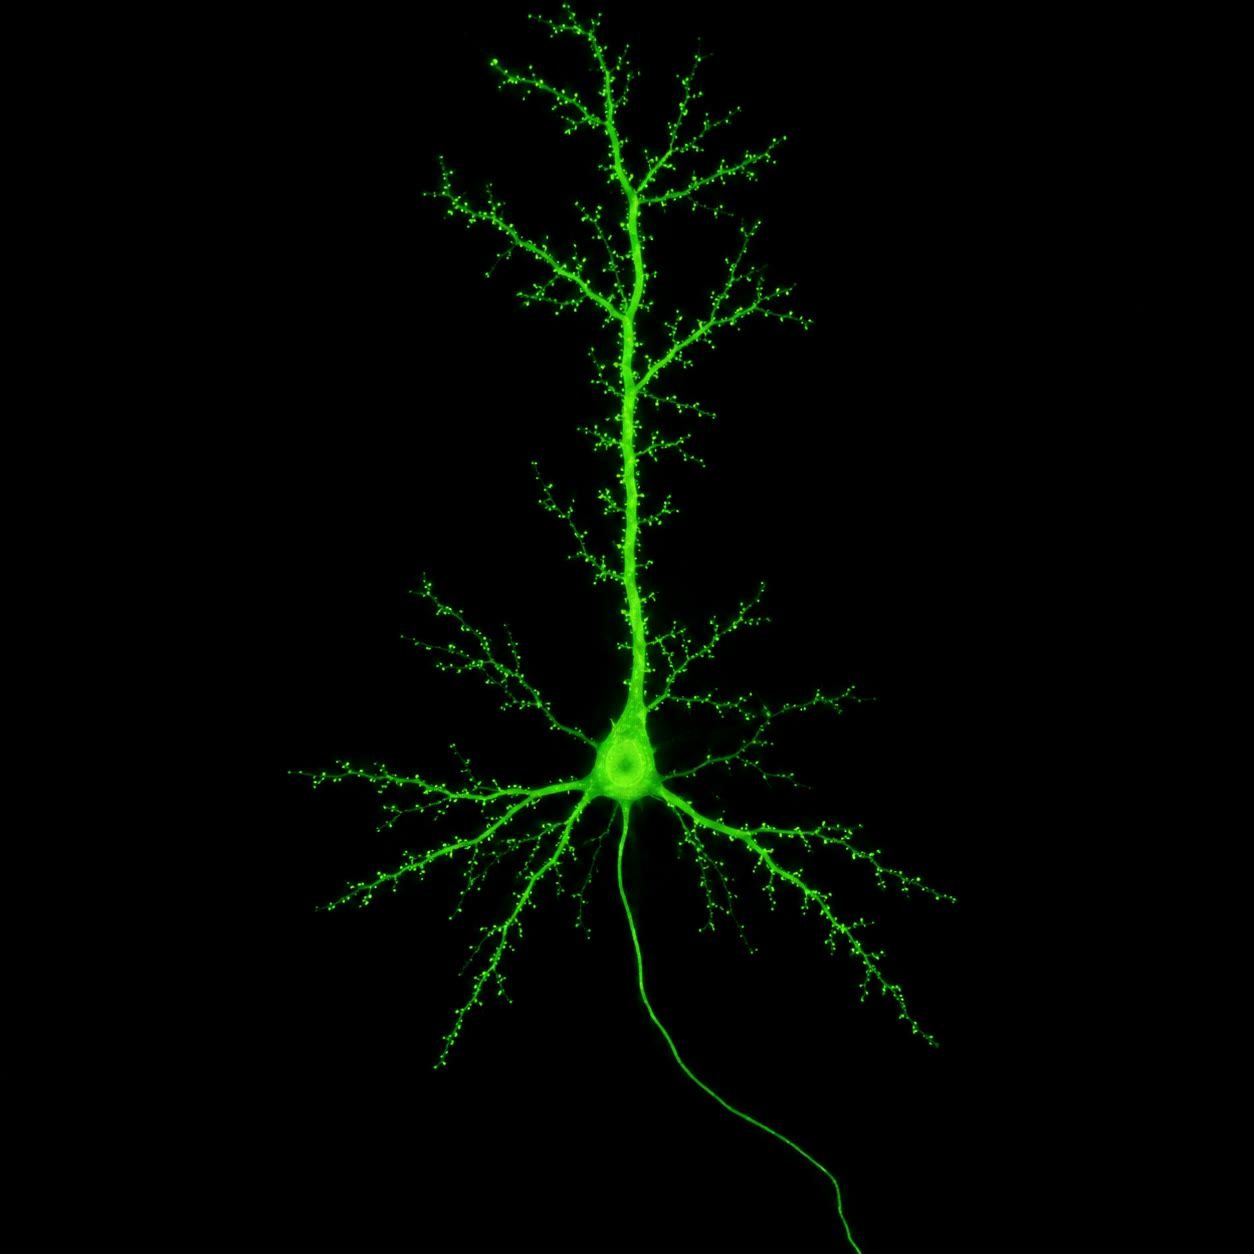
\includegraphics[width=0.4\linewidth]{images/book4/ai/b4-20-neuron-fluorescence.jpg}\hspace{0.05\linewidth}
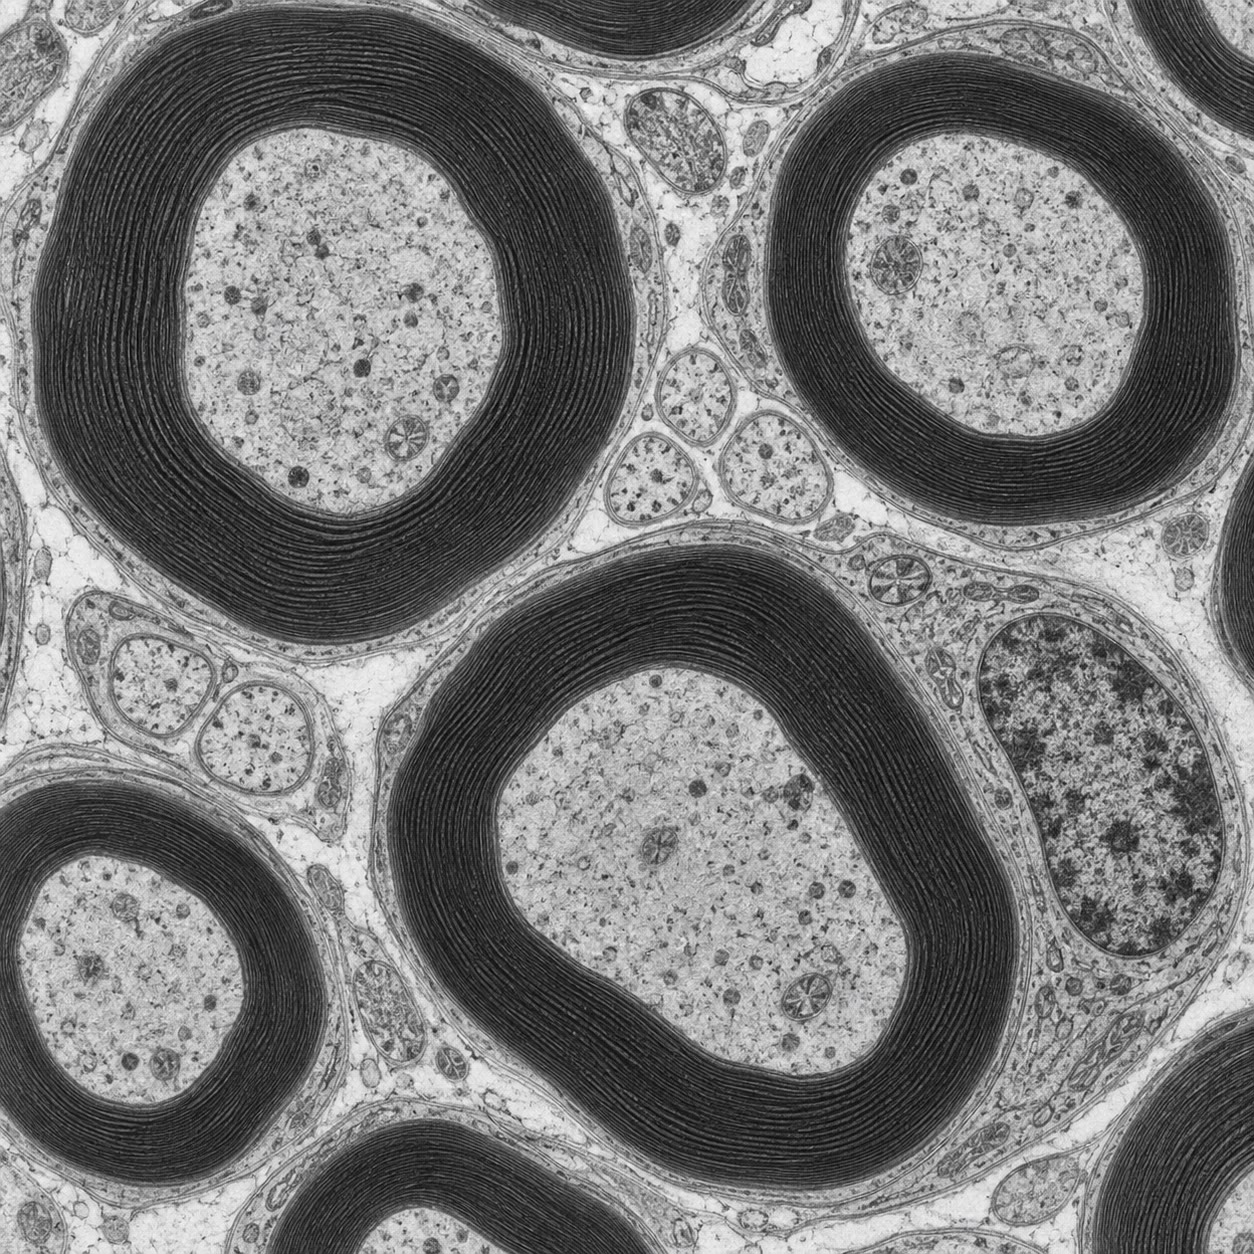
\includegraphics[width=0.4\linewidth]{images/book4/ai/b4-20-myelinated-axons-tem.jpg}

{\small Kiri: sebuah \omterm{def:b2:neurons-synapses:neuron}{neuron} piramid yang diisi zat warna --- badan
selnya, \omterm{def:b2:neurons-synapses:neuron}{dendritnya} yang berduri dan menerima, serta \omterm{def:b2:neurons-synapses:neuron}{aksonnya} yang tipis
dan meninggalkan pangkalnya. Kanan: \omterm{def:b2:neurons-synapses:neuron}{akson} pada penampang lintang di
bawah mikroskop elektron, masing-masing terbungkus pilin gelap seludang
\omterm{def:b2:neurons-synapses:neuron}{mielinnya}.}
\end{omfigure}

\section{Potensial istirahatnya}

\begin{theorem}[Potensial Nernst]\label{thm:b2:neurons-synapses:nernst}
\index{potensial Nernst}\index{potensial kesetimbangan}
Sebuah membran yang telap bagi satu ion bermuatan $z$ yang memisahkan
kepekatan $c_{\text{luar}}$ dan $c_{\text{dalam}}$ mencapai
\emph{\omterm{thm:b2:neurons-synapses:nernst}{potensial kesetimbangan}} yang padanya gaya listrik pada ionnya
mengimbangi difusinya:
\[
E = \frac{RT}{zF}\ln\frac{c_{\text{luar}}}{c_{\text{dalam}}} \approx \frac{\qty{61.5}{mV}}{z}\log_{10}\frac{c_{\text{luar}}}{c_{\text{dalam}}} \quad (\qty{37}{\celsius}).
\]
Sebuah \omterm{def:b2:neurons-synapses:neuron}{neuron} menahan \qty{140}{mmol/L} kalium di dalamnya berbanding
\qty{5}{mmol/L} di luarnya, dan \qty{15}{mmol/L} natrium di dalamnya
berbanding \qty{145}{mmol/L} di luarnya, yaitu landaian yang dibangun
pompa natrium--kalium dengan ongkos sepertiga ATP selnya. Karena itu
$E_{\mathrm K} = 61.5\log_{10}(5/140) = \qty{-89}{mV}$ dan
$E_{\mathrm{Na}} = 61.5\log_{10}(145/15) = \qty{+61}{mV}$: jika
membrannya hanya melewatkan kalium ia akan berada pada \qty{-89}{mV},
jika hanya natrium pada \qty{+61}{mV}.
\end{theorem}
\begin{proof}
Pada kesetimbangan potensial elektrokimia ionnya sama pada kedua
sisinya: $RT\ln c_{\text{dalam}} + zFV_{\text{dalam}} = RT\ln
c_{\text{luar}} + zFV_{\text{luar}}$, sehingga $V_{\text{dalam}} -
V_{\text{luar}} = (RT/zF)\ln(c_{\text{luar}}/c_{\text{dalam}})$. Pada
\qty{310}{K}, $RT/F = \qty{26.7}{mV}$ dan $\ln 10 \times 26.7 =
\qty{61.5}{mV}$. (Diturunkan pada jilid Tahun 1 dari sebaran Boltzmann;
dinyatakan ulang di sini.)
\end{proof}

\begin{theorem}[Potensial istirahat sebagai rerata terbobot]\label{thm:b2:neurons-synapses:chord}
\index{potensial istirahat}\index{konduktans (membran)}
Jika membrannya menghantarkan beberapa ion, masing-masing dengan
konduktans $g_i$ (yaitu kemudahan ia melewatkannya, yang ditetapkan
jumlah kanal yang terbuka), potensial tunak yang padanya arusnya saling
meniadakan adalah
\[
V = \frac{\sum_i g_i E_i}{\sum_i g_i},
\]
yaitu sebuah rerata \omterm{thm:b2:neurons-synapses:nernst}{potensial kesetimbangannya} yang dibobot dengan
konduktansnya. Ketika beristirahat membran sebuah \omterm{def:b2:neurons-synapses:neuron}{neuron} kira-kira dua
puluh kali lebih telap bagi kalium daripada bagi natrium, sehingga $V \approx (20\times(-89) +
61)/21 = \qty{-82}{mV}$; dengan kloridanya dan
rembesan kecilnya ikut dihitung, \omterm{thm:b2:neurons-synapses:chord}{potensial istirahatnya} adalah
\qty{-70}{mV}. Membrannya beristirahat dekat $E_{\mathrm K}$ karena
kanal kaliumnya terbuka; apa pun yang membuka kanal natriumnya
menyeretnya menuju $E_{\mathrm{Na}}$ --- dan itulah seluruh asas
pensinyalan sarafnya.
\end{theorem}
\begin{proof}
Tiap ion membawa arus $I_i = g_i(V - E_i)$ (hukum Ohm, dengan gaya
penggeraknya diukur dari kesetimbangan ionnya sendiri). Pada sebuah
potensial tunak arus totalnya nol: $\sum_i g_i(V - E_i) =
0$, sehingga
$V\sum g_i = \sum g_iE_i$. (Perlakuan penuhnya, yang di dalamnya
ketelapannya masuk lewat persamaan Goldman--Hodgkin--Katz, memberikan
pembobotan yang sama sampai orde pertama.)
\end{proof}

\section{Potensial aksinya}

\begin{proposition}[Impulsnya]\label{prop:b2:neurons-synapses:ap}
\index{potensial aksi}\index{kanal bergerbang tegangan}\index{ambang}\index{masa refrakter}
Membran \omterm{def:b2:neurons-synapses:neuron}{aksonnya} memiliki \emph{kanal natrium bergerbang tegangan},
yang tertutup ketika beristirahat dan dibuka oleh depolarisasi. Jika
sebuah rangsangan menaikkan potensialnya dari \qty{-70}{mV} melewati
sebuah \emph{ambang} yang mendekati \qty{-55}{mV}, cukup banyak
kanalnya membuka untuk memasukkan natrium lebih banyak daripada yang
dapat diimbangi rembesan kaliumnya; potensialnya naik, lebih banyak
kanal membuka, dan dalam sepersekian milidetik membrannya tersapu
menuju $E_{\mathrm{Na}}$ --- sebuah \emph{umpan balik positif} yang
meledak dan bersifat semua-atau-tidak-sama-sekali. Ia memuncak
mendekati \qty{+40}{mV} karena kanal natriumnya
\emph{menonaktifkan diri} dalam semilidetik setelah membuka dan karena
\emph{kanal kalium bergerbang tegangan} yang lebih lambat membuka lalu
menggerakkan potensialnya kembali menuju $E_{\mathrm K}$, dengan
melampaui batasnya menjadi sebuah \emph{ayunan bawah} sebelum kanal
kaliumnya menutup. \emph{\omterm{prop:b2:neurons-synapses:ap}{Potensial aksinya}} berlangsung kira-kira
semilidetik; selama satu atau dua milidetik lagi kanal natriumnya yang
nonaktif tidak dapat membuka kembali (yaitu \emph{\omterm{prop:b2:neurons-synapses:ap}{masa refrakternya}}),
yang membatasi laju picunya menjadi beberapa ratus tiap detik dan
memaksa impulsnya berjalan satu arah. Karena ia bersifat
semua-atau-tidak-sama-sekali, impulsnya tidak membawa keterangan apa
pun dalam ukurannya: \omterm{def:b2:neurons-synapses:neuron}{neuronnya} menyandikan kekuatannya dalam
\emph{frekuensinya}. Sekitar $10^{4}$ ion natrium masuk dan sebanyak
itu pula ion kalium keluar tiap impulsnya --- sebuah perubahan kepekatan
yang dapat diabaikan, yang dipulihkan pompanya dengan santai.
\end{proposition}
\begin{proof}[Bukti eksperimental]
Hodgkin dan Huxley (1952), dengan memakai \omterm{def:b2:neurons-synapses:neuron}{akson} raksasa cumi-cumi
(setebal setengah milimeter, sehingga sehelai kawat dapat diuntaikan di
dalamnya) dan sebuah penguat umpan balik yang menahan potensial
membrannya pada nilai mana pun yang dipilih (yaitu \emph{penjepit
tegangan}) sambil merekam arus yang diperlukan untuk menahannya,
memisahkan arusnya menjadi sebuah komponen masuk yang awal yang lenyap
ketika natriumnya disingkirkan dari rendamannya dan sebuah komponen
keluar yang kemudian yang dibawa kalium; mengukur bagaimana tiap
konduktansnya naik dan turun bersama waktu pada tiap tegangannya; lalu,
dengan mencocokkan masing-masingnya dengan beberapa persamaan,
menghitung bentuk, ambang, kecepatan, dan \omterm{prop:b2:neurons-synapses:ap}{masa refrakter} \omterm{prop:b2:neurons-synapses:ap}{potensial
aksinya} dari kedua konduktansnya saja. Tiap ramalannya bertahan.
Kanalnya sendiri terlihat dua puluh lima tahun kemudian, satu demi
satu, dengan penjepit tampalnya; tetrodotoksin (racun ikan buntal)
menghalangi kanal natriumnya lalu meniadakan impulsnya,
tetraetilamonium menghalangi kanal kaliumnya lalu memperpanjangnya.
\end{proof}

\begin{omfigure}
\begin{tikzpicture}
\begin{axis}[
  width=0.9\linewidth, height=6.4cm,
  axis x line=bottom, axis y line=left,
  xmin=0, xmax=4, ymin=-100, ymax=60,
  xlabel={waktu (ms)}, ylabel={potensial membran (mV)},
  xlabel style={font=\small, at={(axis description cs:0.5,-0.1)}, anchor=north},
  ylabel style={font=\small},
  tick label style={font=\small}, xtick={0,1,2,3,4}, ytick={-90,-70,-55,0,40},
  legend style={font=\scriptsize, at={(0.97,0.95)}, anchor=north east, draw=none},
  clip=false,
]
\addplot[very thick, omDef] coordinates {(0,-70) (0.4,-70) (0.5,-64) (0.6,-55) (0.7,-30) (0.8,10) (0.9,35) (1.0,40) (1.1,30) (1.2,10) (1.35,-20) (1.5,-50) (1.7,-75) (1.9,-85) (2.2,-82) (2.6,-76) (3.2,-71) (4,-70)};
\addlegendentry{potensial membran}
\addplot[thick, omThm, dashed] coordinates {(0,0) (0.5,0) (0.6,5) (0.7,20) (0.8,35) (0.9,30) (1.0,20) (1.1,8) (1.2,3) (1.4,0) (4,0)};
\addlegendentry{$g_{\mathrm{Na}}$ (nisbi)}
\addplot[thick, omProp, dashed] coordinates {(0,0) (0.6,0) (0.8,2) (1.0,8) (1.2,16) (1.4,20) (1.7,17) (2.0,10) (2.4,4) (3.0,1) (4,0)};
\addlegendentry{$g_{\mathrm K}$ (nisbi)}
\draw[dashed, gray] (axis cs:0,-55) -- (axis cs:4,-55); \node[font=\scriptsize, anchor=south east] at (axis cs:4,-55) {ambang};
\draw[dashed, gray] (axis cs:0,-89) -- (axis cs:4,-89); \node[font=\scriptsize, anchor=south east] at (axis cs:3.7,-89) {$E_{\mathrm K}$};
\draw[<->, gray] (axis cs:1.0,50) -- (axis cs:2.5,50); \node[font=\scriptsize, anchor=south, gray] at (axis cs:1.75,50) {refrakter};
\end{axis}
\end{tikzpicture}

{\small Sebuah \omterm{prop:b2:neurons-synapses:ap}{potensial aksi}. Melewati ambangnya konduktans
natriumnya (merah) naik dengan meledak lalu menggerakkan potensialnya
menuju $E_{\mathrm{Na}}$; ia menonaktifkan diri ketika konduktans
kaliumnya (jingga) naik lalu mengembalikan membrannya menuju
$E_{\mathrm K}$, dengan sebuah ayunan bawah. Di bawah garis ambangnya,
tidak ada yang terjadi.}
\end{omfigure}

\section{Penghantaran}

\begin{theorem}[Kabelnya dan tetapan panjangnya]\label{thm:b2:neurons-synapses:cable}
\index{tetapan panjang}\index{persamaan kabel}\index{laju hantar}
Sebuah \omterm{def:b2:neurons-synapses:neuron}{akson} adalah sebuah kabel yang bocor: arus yang disuntikkan pada
sebuah titik mengalir sepanjang sitoplasmanya (hambatan $r_i$ tiap
satuan panjang) lalu bocor keluar lewat membrannya (hambatan $r_m$ kali
satuan panjang). Sebuah depolarisasi tunak $V_0$ pada $x = 0$ meluruh
sepanjang \omterm{def:b2:neurons-synapses:neuron}{aksonnya} sebagai
\[
V(x) = V_0\,e^{-x/\lambda}, \qquad \lambda = \sqrt{\frac{r_m}{r_i}} = \sqrt{\frac{R_m\,d}{4R_i}},
\]
dengan $d$ adalah garis tengahnya dan $R_m$, $R_i$ adalah hambatan
jenis membran dan sitoplasmanya. \emph{\omterm{thm:b2:neurons-synapses:cable}{Tetapan panjang}} $\lambda$
adalah jarak yang padanya sebuah isyarat pasif turun menjadi
sepertiganya: kira-kira \qty{0.5}{mm} bagi sebuah \omterm{def:b2:neurons-synapses:neuron}{akson}
\qty{1}{\micro m}, yang bertambah sebagai akar garis tengahnya. Sebuah
\omterm{prop:b2:neurons-synapses:ap}{potensial aksi} merambat karena depolarisasi pada mukanya, yang menyebar
secara pasif ke depan sejauh kira-kira $\lambda$, membawa ruas membran
berikutnya sampai ambangnya, yang membangkitkannya kembali pada ukuran
penuhnya; makin jauh ke depan ia menjangkau, makin cepat gelombangnya,
sehingga \omterm{thm:b2:neurons-synapses:cable}{laju hantarnya} juga bertambah kira-kira sebagai $\sqrt{d}$ ---
dari \qty{1}{m/s} pada sebuah serabut tipis tanpa \omterm{def:b2:neurons-synapses:neuron}{mielin} menjadi
\qty{20}{m/s} pada \omterm{def:b2:neurons-synapses:neuron}{akson} raksasa cumi-cumi.
\end{theorem}
\begin{proof}
Misalkan $i(x)$ adalah arus aksialnya dan $V(x)$ depolarisasi
membrannya. Hukum Ohm sepanjang aksoplasmanya memberikan $\mathrm{d}V/
\mathrm{d}x = -r_i\,i$; kekekalan muatan, dengan rembesan lewat
membrannya, memberikan $\mathrm{d}i/\mathrm{d}x = -V/r_m$. Dengan
menggabungkannya, $\mathrm{d}^{2}V/\mathrm{d}x^{2} = V/(r_m r_i)$, yang
penyelesaian meluruhnya adalah $V_0 e^{-x/\lambda}$ dengan
$\lambda^{2} = r_m/r_i$. Bagi sebuah silinder, $r_m = R_m/(\pi d)$ dan
$r_i = 4R_i/(\pi d^{2})$, sehingga $\lambda^{2} = R_m d/4R_i$. Dengan
$R_m = \qty{1}{\ohm.m^2}$, $R_i =
\qty{1}{\ohm.m}$ dan $d = \qty{1}{\micro m}$: $\lambda = \sqrt{10^{-6}
/4} = \qty{0.5}{mm}$.
\end{proof}

\begin{proposition}[Mielin dan penghantaran meloncat]\label{prop:b2:neurons-synapses:myelin}
\index{penghantaran meloncat}\index{nodus Ranvier}
\omterm{def:b2:neurons-synapses:neuron}{Mielin} melipatkan $r_m$ dengan jumlah lilitan membrannya dan membagi
kapasitans membrannya dengan faktor yang sama, sehingga di bawah
seludangnya nyaris tidak ada arus yang bocor dan sedikit muatan saja
yang diperlukan untuk mengubah potensialnya: depolarisasinya menyebar
secara pasif sepanjang sebuah antarnodus sepanjang satu milimeter
dengan sedikit rugi, dan \omterm{prop:b2:neurons-synapses:ap}{potensial aksinya} hanya dibangkitkan kembali
pada nodusnya, tempat kanal natriumnya terpusat. Karena itu impulsnya
\emph{meloncat} dari nodus ke nodus (\emph{\omterm{prop:b2:neurons-synapses:myelin}{penghantaran meloncat}}),
pada \qty{100}{m/s} di dalam sebuah serabut \qty{20}{\micro m} ---
sebuah kecepatan yang untuk mencapainya sebuah \omterm{def:b2:neurons-synapses:neuron}{akson} tanpa \omterm{def:b2:neurons-synapses:neuron}{mielin} harus
setebal beberapa sentimeter --- dan dengan sepersekian ongkos
metabolisnya, karena natriumnya hanya masuk pada nodusnya. \omterm{def:b2:neurons-synapses:neuron}{Mielin}
adalah temuan vertebrata yang memungkinkan sebuah sistem saraf yang
besar dan cepat di dalam sebuah tubuh yang kecil; pada sklerosis
ganda seludangnya dimusnahkan petak demi petak, \omterm{thm:b2:neurons-synapses:cable}{tetapan panjangnya}
runtuh, dan impulsnya gagal.
\end{proposition}

\begin{omfigure}
\begin{tikzpicture}[every node/.style={font=\scriptsize}, >=stealth]
  % unmyelinated
  \begin{scope}
    \draw[thick, fill=omDef!10] (0,0) rectangle (11,0.5);
    \foreach \x in {0.5,1.0,...,10.5} \draw[omThm, ->] (\x,0.25) -- (\x,0.9);
    \node[anchor=east] at (-0.2,0.25) {tanpa mielin};
    \node[anchor=west] at (11.2,0.25) {\qty{1}{m/s}};
    \node[above] at (5.5,1.0) {impulsnya dibangkitkan kembali pada tiap titiknya};
  \end{scope}
  % myelinated
  \begin{scope}[yshift=-2.4cm]
    \draw[thick, fill=omDef!10] (0,0) rectangle (11,0.5);
    \foreach \x in {0.3,2.5,4.7,6.9,9.1} \fill[omExo!60] (\x,-0.15) rectangle (\x+1.9,0.65);
    \foreach \x in {2.35,4.55,6.75,8.95} \draw[omThm, ->] (\x,0.25) -- (\x,0.9);
    \foreach \x in {2.35,4.55,6.75} \draw[->, thick, omThm, dashed] (\x+0.1,1.1) .. controls (\x+1.1,1.6) .. (\x+2.1,1.1);
    \node[anchor=east] at (-0.2,0.25) {bermielin};
    \node[anchor=west] at (11.2,0.25) {\qty{100}{m/s}};
    \node[below] at (1.25,-0.2) {antarnodus mielin};
    \node[below] at (4.55,-0.2) {nodus Ranvier};
    \node[above] at (5.5,1.6) {dibangkitkan kembali hanya pada nodusnya: meloncat};
  \end{scope}
\end{tikzpicture}

{\small Penghantaran dengan dan tanpa \omterm{def:b2:neurons-synapses:neuron}{mielin}. Di dalam sebuah \omterm{def:b2:neurons-synapses:neuron}{akson}
telanjang impulsnya dibangkitkan kembali di sepanjangnya; di bawah
\omterm{def:b2:neurons-synapses:neuron}{mielin} isyaratnya menyebar secara pasif sepanjang tiap antarnodusnya
lalu dibangkitkan kembali pada nodusnya, dan impulsnya berjalan seratus
kali lebih cepat.}
\end{omfigure}

\section{Sinapsisnya}

\begin{definition}[Sinapsis kimia dan sinapsis listrik]\label{def:b2:neurons-synapses:synapse}
\index{sinapsis}\index{neurotransmiter}\index{potensial pascasinapsis}
Pada sebuah \emph{sinapsis} terminal sebuah \omterm{def:b2:neurons-synapses:neuron}{neuron} berjumpa dengan
sebuah sasaran --- sebuah \omterm{def:b2:neurons-synapses:neuron}{neuron} lain, sebuah \omterm{def:b2:cell-differentiation:myogenesis}{serabut otot}, sebuah sel
kelenjar. Pada sinapsis \emph{listrik} sambungan renggang menyatukan
kedua selnya dan arusnya lewat secara langsung --- cepat, dua arah,
tanpa penguatan, dipakai di tempat kecepatan dan keserentakan berarti
(refleks lolos, \omterm{def:b2:heart:anatomy}{jantungnya}). Pada sinapsis \emph{kimia} selnya
dipisahkan sebuah celah \qty{20}{nm} dan isyaratnya adalah sebuah
molekul. Sebuah \omterm{prop:b2:neurons-synapses:ap}{potensial aksi} yang tiba di terminalnya membuka kanal
kalsium bergerbang tegangan; kalsiumnya masuk lalu, dalam sepersekian
milidetik, membuat vesikel berisi \emph{neurotransmiter} melebur dengan
membrannya lalu mengosongkan diri ke dalam celahnya; penghantarnya
berdifusi menyeberang dalam hitungan mikrodetik lalu mengikat reseptor
pada membran pascasinapsisnya --- entah kanal ion yang ia buka
(\emph{ionotropik}, cepat) atau \omterm{prop:b2:cell-signalling:gpcr}{reseptor berpasangan protein G}
(\emph{metabotropik}, lebih lambat, \cref{ch:b2:cell-signalling});
arus yang dihasilkannya menggeser potensial pascasinapsisnya beberapa
milivolt, naik (sebuah \emph{potensial pascasinapsis perangsang}, dari
kanal yang melewatkan natrium) atau turun (sebuah potensial
\emph{penghambat}, dari kanal yang melewatkan klorida atau kalium); dan
penghantarnya disingkirkan dalam hitungan milidetik oleh sebuah enzim
atau sebuah pengangkut. Tundaannya setengah milidetik; harganya membeli
penghantaran satu arah, penguatan, penghambatan, dan keterubahan ---
segala yang diperlukan sebuah sistem saraf di luar penghantaran belaka.
\end{definition}

\begin{omfigure}
\begin{tikzpicture}[every node/.style={font=\scriptsize}, >=stealth]
  % presynaptic terminal
  \draw[thick, fill=omDef!10] (0,0) .. controls (0,2.6) and (3.6,2.6) .. (3.6,0.2) -- (3.6,-0.2) .. controls (3.6,-2.6) and (0,-2.6) .. (0,0);
  \draw[very thick, omDef] (-2.2,0) -- (0.1,0); \node[omDef, above] at (-1.1,0.05) {akson};
  \foreach \p in {(2.0,1.0),(2.6,0.5),(2.7,-0.4),(2.1,-1.0),(1.6,0.2)} \draw[thick, fill=omProp!40] \p circle (0.25);
  \draw[thick, fill=omProp!40] (3.3,0.1) arc (90:-90:0.25) -- cycle;
  \foreach \p in {(3.75,0.2),(3.85,-0.1),(3.7,-0.35),(3.9,0.4)} \fill[omProp] \p circle (0.05);
  \fill[omThm] (3.45,1.3) circle (0.06); \node[omThm, anchor=east] at (3.35,1.45) {Ca$^{2+}$ masuk};
  \draw[->, omThm] (3.9,1.5) -- (3.55,1.35);
  % cleft
  \node[align=center, anchor=north] at (3.85,-2.75) {celah\\\qty{20}{nm}};
  \draw[gray] (3.85,-2.7) -- (3.85,-1.2);
  % postsynaptic
  \draw[thick, fill=omExo!15] (4.1,-2.6) rectangle (8.2,2.6);
  \foreach \y in {0.9,0.3,-0.3,-0.9} \draw[thick, fill=omDef!40] (4.05,\y-0.15) rectangle (4.45,\y+0.15);
  \node[anchor=west, align=left] at (4.6,0.3) {reseptor: kanal\\membuka, ion mengalir,\\potensial\\pascasinapsis};
  \node[anchor=west, align=left] at (4.6,-1.7) {penghantar disingkirkan\\oleh enzim atau\\pengangkut};
  \node[anchor=west] at (4.6,2.2) {sel pascasinapsis};
  % labels
  \node[align=center, anchor=north] at (1.8,-2.75) {vesikel berisi\\penghantar};
  \node[anchor=south] at (1.8,2.75) {terminal prasinapsis};
\end{tikzpicture}

{\small Sebuah \omterm{def:b2:neurons-synapses:synapse}{sinapsis} kimia. Impulsnya memasukkan kalsium, vesikelnya
melebur lalu melepaskan penghantarnya ke dalam celahnya, reseptor pada
sasarannya membuka kanal, dan penghantarnya dibersihkan dalam hitungan
milidetik.}
\end{omfigure}

\begin{theorem}[Pelepasan kuantal]\label{thm:b2:neurons-synapses:quantal}
\index{pelepasan kuantal}\index{potensial mini}
Penghantarnya dilepaskan dalam paket --- \emph{kuantum}, masing-masing
satu vesikel --- dan jumlah $k$ yang dilepaskan satu impuls adalah
sebuah peubah acak. Jika terminalnya memiliki $n$ tapak pelepasan yang
masing-masing melepaskan dengan peluang $p$, dan $p$ kecil, maka $k$
kira-kira berdistribusi Poisson dengan rerata $m = np$:
\[
P(k) = \frac{m^{k}e^{-m}}{k!}, \qquad P(0) = e^{-m}, \qquad
m = \ln\frac{\text{jumlah percobaan}}{\text{jumlah kegagalan}}.
\]
Karena itu isi kuantal rerata $m$ dapat dibaca dari bagian impuls yang
tidak melepaskan apa pun, lalu diperiksa terhadap tanggapan reratanya
dibagi ukuran satu kuantumnya. Pada sebuah \omterm{prop:b2:neurons-synapses:integration}{sambungan saraf-otot} $m$
bernilai beberapa ratus --- penghantarannya tidak pernah gagal; pada
sebuah \omterm{def:b2:neurons-synapses:synapse}{sinapsis} pusat nilainya sering mendekati satu, dan \omterm{def:b2:neurons-synapses:synapse}{sinapsisnya}
menghantar pada sebagian kecil impulsnya.
\end{theorem}
\begin{proof}
Dengan $n$ tapak bebas yang masing-masing melepaskan dengan peluang
$p$, $k$ berdistribusi binomial; bagi $n$ yang besar dan $p$ yang kecil
dengan $np = m$ tetap, binomialnya menuju hukum Poisson (seri
matematika, Tahun 2). $P(0) = e^{-m}$ memberikan $m$ dari
kegagalannya. Pemeriksaan Katz adalah bahwa $m$ yang sama, yang
dimasukkan ke rumus Poissonnya, meramalkan bagian tanggapan satu, dua,
dan tiga kuantum yang teramati.
\end{proof}
\begin{proof}[Bukti eksperimental]
Fatt dan Katz (1952) merekam dari sebuah \omterm{def:b2:cell-differentiation:myogenesis}{serabut otot} katak yang
beristirahat depolarisasi spontan kecil sebesar kira-kira
\qty{0.5}{mV}, yang semuanya berukuran sama, pada selang waktu yang
acak --- yaitu \emph{potensial lempeng-ujung mini}, yang
masing-masingnya adalah efek satu vesikel. Menurunkan kalsium di dalam
rendamannya mengurangi tanggapan terhadap perangsangan sarafnya sampai
tanggapannya bergoyang di antara 0, 1, 2, atau 3 kelipatan ukuran
mininya; frekuensi kelipatannya mengikuti hukum Poisson dengan $m$ yang
dihitung dari kegagalannya. Del Castillo dan Katz dengan demikian
menunjukkan bahwa pelepasannya bersifat kuantal, bahwa kalsium
mengendalikan peluang pelepasannya dan bukan ukuran sebuah kuantumnya,
dan mikroskopi elektron memperlihatkan vesikel yang menjadi kuantumnya.
\end{proof}

\begin{proposition}[Pemaduan: neuron sebagai sebuah keputusan]\label{prop:b2:neurons-synapses:integration}
\index{penjumlahan}\index{bukit akson}\index{sambungan saraf-otot}
Sebuah \omterm{def:b2:neurons-synapses:neuron}{neuron} pusat menerima ribuan \omterm{def:b2:neurons-synapses:synapse}{sinapsis}, yang merangsang maupun
yang menghambat, pada \omterm{def:b2:neurons-synapses:neuron}{dendrit} dan somanya. Tiap \omterm{def:b2:neurons-synapses:synapse}{potensial
pascasinapsisnya} kecil dan meluruh secara pasif, dengan \omterm{thm:b2:neurons-synapses:cable}{tetapan panjang}
kabelnya dalam ruang dan tetapan waktu membrannya (beberapa milidetik)
dalam waktu; potensialnya berjumlah --- \emph{penjumlahan ruang} bagi
masukan yang tiba bersama-sama, \emph{penjumlahan waktu} bagi masukan
yang tiba berturut-turut dengan cepat --- dan jumlahnya dibaca pada
\emph{\omterm{prop:b2:neurons-synapses:integration}{bukit aksonnya}}, tempat kanal natriumnya paling rapat dan
ambangnya paling rendah. Jika jumlahnya melewati ambangnya \omterm{def:b2:neurons-synapses:neuron}{aksonnya}
memicu, pada laju yang naik bersama kelebihannya; masukan yang
menghambat mengurangi, dan sebuah \omterm{def:b2:neurons-synapses:synapse}{sinapsis} penghambat yang dekat dengan
bukitnya dapat memveto sebuah \omterm{def:b2:neurons-synapses:synapse}{sinapsis} perangsang yang jauh. \omterm{prop:b2:neurons-synapses:integration}{Sambungan
saraf-ototnya} adalah kekecualian yang memperlihatkan kaidahnya: satu
terminal motorik, yang melepaskan ratusan kuantum asetilkolin ke atas
reseptor yang sekaligus merupakan kanalnya, memberikan sebuah potensial
lempeng-ujung sebesar \qty{50}{mV}, yang jauh di atas ambangnya --- tiap
impuls di dalam saraf motoriknya menghasilkan sebuah \omterm{prop:b2:neurons-synapses:ap}{potensial aksi} otot
(\cref{ch:b2:muscle-movement}). Kurare, yang menghalangi reseptornya,
melumpuhkan; gas saraf, yang menghalangi enzim yang menyingkirkan
asetilkolinnya, melumpuhkan lewat kelebihan yang berlawanan.
\end{proposition}

\begin{example}[Penghantar dan obat]\label{ex:b2:neurons-synapses:transmitters}
Asetilkolin pada \omterm{prop:b2:neurons-synapses:integration}{sambungan saraf-otot} dan di dalam sistem otonomnya;
glutamat, yaitu penghantar perangsang utama otaknya, dan GABA, yaitu
penghantar penghambat utamanya; monoamina noradrenalin, dopamin, dan
serotonin, yang menyelia seluruh untaian dari beberapa ribu sel saja;
serta berlusin-lusin peptida. Hampir tiap obat yang bekerja pada
pikirannya bekerja pada sebuah \omterm{def:b2:neurons-synapses:synapse}{sinapsis}: benzodiazepina menguatkan
kanal GABA-nya, antidepresan menghalangi pengangkut serotoninnya,
kokaina menghalangi pengangkut dopaminnya, opiat meniru sebuah peptida,
nikotina meniru asetilkolin pada satu reseptor dan atropin
menghalanginya pada reseptor lain, toksin botulinum memotong protein
yang meleburkan vesikelnya. \omterm{def:b2:neurons-synapses:synapse}{Sinapsisnya} adalah tempat kimia pada
\cref{ch:b2:cell-signalling} dan kelistrikan pada bab ini berjumpa, dan
tempat sebuah sistem saraf belajar: \omterm{def:b2:neurons-synapses:synapse}{sinapsis} yang dipakai menguat, dan
penguatan itu (jilid Tahun 3) adalah ingatan.
\end{example}

\section{Latihan}

\begin{exercise}[$\star$]\label{exo:b2:neurons-synapses:1}
Sebutkan bagian sebuah \omterm{def:b2:neurons-synapses:neuron}{neuron} dan fungsi masing-masingnya, lalu
katakan \omterm{def:b2:neurons-synapses:neuron}{mielinnya} terbuat dari apa dan apa yang ia kerjakan.
\end{exercise}

\begin{exercise}[$\star$]\label{exo:b2:neurons-synapses:2}
Perikanlah fase sebuah \omterm{prop:b2:neurons-synapses:ap}{potensial aksi} dan peristiwa kanal yang
menyebabkan masing-masingnya. Mengapa ia bersifat
semua-atau-tidak-sama-sekali, dan mengapa ia tidak berjalan mundur?
\end{exercise}

\begin{exercise}[$\star$]\label{exo:b2:neurons-synapses:3}
Sebutkan langkah penghantaran pada sebuah \omterm{def:b2:neurons-synapses:synapse}{sinapsis} kimia dari tibanya
impulsnya sampai disingkirkannya penghantarnya.
\end{exercise}

\begin{exercise}[$\star$]\label{exo:b2:neurons-synapses:4}
Bandingkan \omterm{def:b2:neurons-synapses:synapse}{sinapsis} listrik dan \omterm{def:b2:neurons-synapses:synapse}{sinapsis} kimia dalam hal kecepatan,
arah, penguatan, dan kemungkinan penghambatannya.
\end{exercise}

\begin{exercise}[$\star\star$]\label{exo:b2:neurons-synapses:5}
Hitunglah \omterm{thm:b2:neurons-synapses:nernst}{potensial Nernst} pada \qty{37}{\celsius} bagi kalium (140 di
dalam, 5 di luar), natrium (15 di dalam, 145 di luar), klorida (10 di
dalam, 110 di luar), dan kalsium (\qty{1e-4}{} di dalam, 2 di luar,
dalam \unit{mmol/L}). Ke arah mana tiap ionnya mengalir ketika
membrannya berada pada \qty{-70}{mV}?
\end{exercise}

\begin{exercise}[$\star\star$]\label{exo:b2:neurons-synapses:6}
Dengan $E_{\mathrm K} = \qty{-89}{mV}$ dan $E_{\mathrm{Na}} =
\qty{+61}{mV}$, hitunglah potensial membrannya ketika $g_{\mathrm K} :
g_{\mathrm{Na}} = 20 : 1$ (istirahat), $1 : 20$ (puncak impulsnya), dan
$50 : 1$ (ayunan bawahnya). Jelaskan tiap keadaannya.
\end{exercise}

\begin{exercise}[$\star\star$]\label{exo:b2:neurons-synapses:7}
\omterm{thm:b2:neurons-synapses:cable}{Laju hantar} berskala sebagai $\sqrt d$ pada \omterm{def:b2:neurons-synapses:neuron}{akson} tanpa \omterm{def:b2:neurons-synapses:neuron}{mielin}, dengan
\qty{1}{m/s} pada \qty{1}{\micro m}. Hitunglah laju sebuah \omterm{def:b2:neurons-synapses:neuron}{akson}
cumi-cumi \qty{0.5}{mm}. Sebuah serabut bermielin \qty{20}{\micro m}
menghantar pada \qty{100}{m/s}: seberapa tebal sebuah \omterm{def:b2:neurons-synapses:neuron}{akson} tanpa
\omterm{def:b2:neurons-synapses:neuron}{mielin} harus dibuat untuk menyamainya? Berapa lama sebuah impuls
memerlukan waktu dari sumsum tulang belakangnya sampai jari kakinya
(\qty{1}{m}) pada tiap serabutnya?
\end{exercise}

\begin{exercise}[$\star\star$]\label{exo:b2:neurons-synapses:8}
Pada 200 perangsangan sebuah \omterm{def:b2:neurons-synapses:synapse}{sinapsis} di dalam kalsium yang rendah, 74
tidak menghasilkan tanggapan. Hitunglah isi kuantal reratanya dan
bagian tanggapan satu, dua, dan tiga kuantum yang diramalkan. Kuantum
tunggalnya adalah \qty{0.5}{mV}: tanggapan rerata berapa yang
diharapkan?
\end{exercise}

\begin{exercise}[$\star\star$]\label{exo:b2:neurons-synapses:9}
\omterm{prop:b2:neurons-synapses:ap}{Masa refrakter} sebuah \omterm{def:b2:neurons-synapses:neuron}{neuron} adalah \qty{2}{ms}. Berapakah laju
picunya yang maksimal? Sebuah \omterm{def:b2:neurons-synapses:neuron}{neuron} sensorik memicu pada 20 impuls
tiap detik bagi sebuah sentuhan ringan dan 200 bagi sentuhan yang
keras: apa yang disandikan, dan oleh apa?
\end{exercise}

\begin{exercise}[$\star\star\star$]\label{exo:b2:neurons-synapses:10}
Hitunglah \omterm{thm:b2:neurons-synapses:cable}{tetapan panjangnya} bagi $R_m = \qty{1}{\ohm.m^2}$, $R_i =
\qty{1}{\ohm.m}$, dan garis tengah 1, 10, dan \qty{500}{\micro m}.
\omterm{def:b2:neurons-synapses:neuron}{Mielin} melipatkan $R_m$ dengan 200: hitung ulang bagi \qty{10}{\micro
m}. Jelaskan mengapa sebuah antarnodus \qty{1}{mm} berhasil dan mengapa
sebuah ruas tanpa \omterm{def:b2:neurons-synapses:neuron}{mielin} sepanjang \qty{3}{mm} menghalangi impulsnya.
\end{exercise}

\begin{exercise}[$\star\star\star$]\label{exo:b2:neurons-synapses:11}
Ramalkan efeknya pada \omterm{prop:b2:neurons-synapses:ap}{potensial aksinya} dan pada penghantaran di
\omterm{prop:b2:neurons-synapses:integration}{sambungan saraf-ototnya} dari: tetrodotoksin; tetraetilamonium; sebuah
rendaman tanpa kalsium; kurare; sebuah penghambat asetilkolinesterase;
toksin botulinum.
\end{exercise}

\begin{exercise}[$\star\star\star$]\label{exo:b2:neurons-synapses:12}
``Sebuah \omterm{def:b2:neurons-synapses:synapse}{sinapsis} kimia berongkos setengah milidetik dan membeli sebuah
sistem saraf.'' Bahaslah apa yang dibayar tundaannya --- penghantaran
satu arah, penguatan, penghambatan, keplastisan --- dan di mana tubuhnya
memakai \omterm{def:b2:neurons-synapses:synapse}{sinapsis} listrik sebagai gantinya.
\end{exercise}

\section{Soal: Sentakan Lutut Diukur Waktunya}

\begin{problem}[{Soal akhir pekan --- refleks regang diikuti dari
ketukan tendonnya sampai tendangannya, dengan potensial istirahat
neuronnya dihitung, waktu penghantaran impulsnya diukur sepanjang kedua
tungkai busurnya, isi kuantal sinapsisnya diukur, dan seluruh
tundaannya diterangkan, berakhir pada potensial istirahatnya, waktu
penghantarannya, isi kuantalnya, dan tundaan refleksnya}]
\label{pb:b2:neurons-synapses:1}
Data pada \qty{37}{\celsius}: kalium 140 di dalam, 4 di luar; natrium
12 di dalam, 145 di luar (\unit{mmol/L}); $g_{\mathrm K} : g_{\mathrm{Na}} = 25 : 1$
ketika beristirahat. \omterm{def:b2:neurons-synapses:neuron}{Akson} sensorik dan motoriknya: \qty{15}{\micro m},
bermielin, \qty{90}{m/s}, \qty{0.9}{m} tiap arahnya. Tundaan
\omterm{def:b2:neurons-synapses:synapse}{sinapsisnya} \qty{0.6}{ms}; pengaktifan ototnya setelah \omterm{prop:b2:neurons-synapses:ap}{potensial
aksinya} sendiri \qty{5}{ms}. \omterm{def:b2:neurons-synapses:synapse}{Sinapsis} pusatnya di dalam kalsium yang
rendah: 300 percobaan, 111 kegagalan. Kuantumnya \qty{0.4}{mV};
ambangnya \qty{15}{mV} di atas istirahatnya. $R_m =
\qty{1}{\ohm.m^2}$, $R_i = \qty{1}{\ohm.m}$; \omterm{def:b2:neurons-synapses:neuron}{mielinnya} melipatkan $R_m$
dengan 250.

\medskip
\noindent\textbf{Bagian I --- \omterm{def:b2:neurons-synapses:neuron}{Neuron} yang beristirahat.}
\begin{enumerate}
  \item Hitunglah $E_{\mathrm K}$ dan $E_{\mathrm{Na}}$.
  \item Hitunglah \omterm{thm:b2:neurons-synapses:chord}{potensial istirahatnya} dari nisbah konduktansnya.
  \item Kalium di luar selnya naik menjadi \qty{8}{mmol/L} (seperti
        setelah olahraga yang berat). Hitung ulang $E_{\mathrm K}$ dan
        \omterm{thm:b2:neurons-synapses:chord}{potensial istirahatnya}, lalu katakan apa yang dikerjakan hal
        ini terhadap keterangsangannya.
  \item Pompanya berhenti. Jelaskan apa yang terjadi pada landaiannya
        dan potensialnya selama berjam-jam, dan mengapa selnya
        menggembung.
  \item Berapa banyak ion natrium yang masuk ke sebuah \omterm{def:b2:neurons-synapses:neuron}{akson}
        \qty{15}{\micro m} tiap milimeter tiap impulsnya jika
        kapasitans membrannya \qty{0.01}{F/m^2} dan potensialnya
        berayun sebesar \qty{100}{mV}? ($Q = CV$; satu ion membawa
        \qty{1.6e-19}{C}.)
  \item Dengan bagian berapa hal itu mengubah kepekatan natrium di
        dalamnya (volume \omterm{def:b2:neurons-synapses:neuron}{aksonnya} tiap milimeter)?
  \item Pompanya mengekspor tiga ion natrium tiap ATP. Berapa banyak
        ATP yang diperlukan untuk membatalkan satu impuls tiap
        milimeter \omterm{def:b2:neurons-synapses:neuron}{aksonnya}?
\end{enumerate}

\medskip
\noindent\textbf{Bagian II --- Penghantaran.}
\begin{enumerate}[resume]
  \item Hitunglah waktu bagi impuls sensoriknya untuk mencapai sumsum
        tulang belakangnya dan bagi impuls motoriknya untuk mencapai
        ototnya.
  \item Hitunglah \omterm{thm:b2:neurons-synapses:cable}{tetapan panjang} sebuah \omterm{def:b2:neurons-synapses:neuron}{akson} \qty{15}{\micro m} yang
        telanjang dan \omterm{def:b2:neurons-synapses:neuron}{akson} yang sama di bawah \omterm{def:b2:neurons-synapses:neuron}{mielinnya}.
  \item Sebuah antarnodus panjangnya \qty{1.5}{mm}. Bagian berapa dari
        depolarisasi nodusnya yang mencapai nodus berikutnya secara
        pasif, dengan dan tanpa \omterm{def:b2:neurons-synapses:neuron}{mielinnya}? Keadaan yang mana yang dapat
        membawa nodus berikutnya sampai ambangnya (\qty{15}{mV} dari
        sebuah impuls \qty{100}{mV})?
  \item Tanpa \omterm{def:b2:neurons-synapses:neuron}{mielin}, \omterm{def:b2:neurons-synapses:neuron}{akson} yang sama akan menghantar pada $\sqrt{15}$
        m/s. Hitunglah perjalanan bolak-baliknya lalu berilah ulasan.
  \item Sepetak \qty{4}{mm} kehilangan \omterm{def:b2:neurons-synapses:neuron}{mielinnya}. Hitunglah bagian
        isyarat yang menyeberanginya lalu katakan apakah refleksnya
        bertahan.
  \item Mengapa \omterm{prop:b2:neurons-synapses:ap}{masa refrakternya} membuat impulsnya berjalan hanya
        satu arah di sepanjang \omterm{def:b2:neurons-synapses:neuron}{akson} sensoriknya?
\end{enumerate}

\medskip
\noindent\textbf{Bagian III --- \omterm{def:b2:neurons-synapses:synapse}{Sinapsisnya}.}
\begin{enumerate}[resume]
  \item Hitunglah isi kuantal rerata $m$ dari kegagalannya.
  \item Hitunglah bagian tanggapan 1, 2, dan 3 kuantum yang
        diramalkan, dan jumlah yang diharapkan di antara 300
        percobaannya.
  \item Hitunglah \omterm{def:b2:neurons-synapses:synapse}{potensial pascasinapsis} reratanya.
  \item Di dalam kalsium yang normal \omterm{def:b2:neurons-synapses:synapse}{sinapsis} yang sama memiliki
        $m = 60$. Berapakah peluang sebuah kegagalannya, dan tanggapan
        reratanya? Apakah satu \omterm{def:b2:neurons-synapses:synapse}{sinapsis} semacam itu memicu \omterm{def:b2:neurons-synapses:neuron}{neuron}
        motoriknya?
  \item \omterm{def:b2:neurons-synapses:neuron}{Neuron} motoriknya menerima \num{20} \omterm{def:b2:neurons-synapses:synapse}{sinapsis} sensorik semacam
        itu yang aktif sekaligus. Jelaskan bagaimana \omterm{def:b2:neurons-synapses:synapse}{sinapsisnya}
        berjumlah dan apakah ambangnya tercapai.
  \item Sebuah \omterm{def:b2:neurons-synapses:synapse}{sinapsis} penghambat pada \omterm{def:b2:neurons-synapses:neuron}{neuron} yang sama membuka kanal
        klorida ($E_{\mathrm{Cl}} = \qty{-70}{mV}$, yaitu \omterm{thm:b2:neurons-synapses:chord}{potensial
        istirahatnya}). Jelaskan bagaimana ia dapat mengurangi tanggapan
        perangsangnya tanpa menghiperpolarisasi selnya.
\end{enumerate}

\medskip
\noindent\textbf{Bagian IV --- Seluruh refleksnya.}
\begin{enumerate}[resume]
  \item Jumlahkan: penghantaran sensoriknya, tundaan \omterm{def:b2:neurons-synapses:synapse}{sinapsisnya},
        penghantaran motoriknya, tundaan saraf-ototnya (\qty{0.6}{ms}),
        dan pengaktifan ototnya. Bandingkan dengan \qty{30}{ms} yang
        terukur.
  \item Dari mana sisa tundaan yang terukur itu berasal?
  \item Refleksnya memiliki satu \omterm{def:b2:neurons-synapses:synapse}{sinapsis} (monosinaptik). Jelaskan
        mengapa sebuah refleks menarik diri, yang memiliki dua atau
        tiga \omterm{def:b2:neurons-synapses:synapse}{sinapsis} di dalam sumsumnya, lebih lambat tetapi lebih
        luwes.
  \item Ketukan yang sama pada seorang pasien dengan penghilangan
        \omterm{def:b2:neurons-synapses:neuron}{mielin} tepi memberikan sebuah refleks yang terlambat
        \qty{60}{ms}. Taksirlah \omterm{thm:b2:neurons-synapses:cable}{laju hantar} di dalam sarafnya.
  \item Sebuah takaran tetrodotoksin menghalangi separuh kanal
        natriumnya. Ramalkan efeknya pada ambangnya, impulsnya, dan
        refleksnya.
  \item Nyatakan hasilnya: \omterm{thm:b2:neurons-synapses:chord}{potensial istirahatnya}, waktu penghantaran
        sensorik dan motoriknya, isi kuantal $m$-nya, dan tundaan
        refleks yang dihitung.
\end{enumerate}
\end{problem}
